% Euclidean Handout Number Eighteen
\documentclass{tufte-handout}

%\geometry{showframe}% for debugging purposes -- displays the margins

%%%% Packages to make things pretty
\usepackage{amsmath,amsthm}
\usepackage{booktabs}
\usepackage{graphicx}
\setkeys{Gin}{width=\linewidth,totalheight=\textheight,keepaspectratio}
\graphicspath{{graphics/}}
\usepackage{units}
\usepackage{fancyvrb}
\fvset{fontsize=\normalsize}
\usepackage{multicol}
\usepackage{pdfpages}

%%%% Theorem Evironments
\theoremstyle{definition}
\swapnumbers
\newtheorem{problem}{Problem}[section]
\newtheorem{conjecture}[problem]{Conjecture}
\newtheorem*{definition}{Definition}
\newtheorem*{theorem}{Theorem}
\newtheorem{question}[problem]{Question}
\newtheorem{challenge}[problem]{Challenge}
\newtheorem*{postulate}{Postulate}

%%%%%

\title{Euclidean Geometry:\\An Introduction to Mathematical Work}
\author[]{Math 3600}
\date{Spring 2015}

\begin{document}

\maketitle

\begin{marginfigure}
    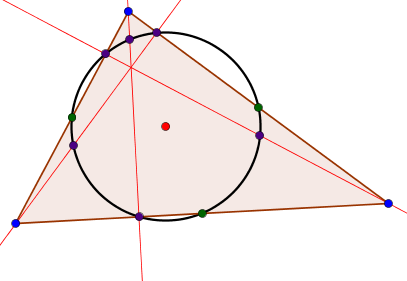
\includegraphics{NPC}
\end{marginfigure}

\setcounter{section}{18}
\section{The Nine Point Circle}


\begin{definition} Let $ABC$ be a triangle with orthocenter $H$. Let $e_A$, $e_B$ and $e_C$ be the midpoints of the segments $AH$, $BH$ and $CH$, respectively. These three points are called the \emph{Euler points} of triangle $ABC$.
\end{definition}

\begin{problem} Let $ABC$ be a triangle with Euler points $e_A$, $e_B$ and $e_C$. Show that the triangle $e_A e_B e_C$ has the same orthocenter as triangle $ABC$.
\end{problem}

\begin{problem}[The Nine-Point Circle]\label{prob:nine-pt-circle}
Let $ABC$ be a triangle. Let $D, E, F$ be the midpoints of the sides, and $H$ the orthocenter. Let $e_A, e_B$ and $e_C$ be the Euler points of $ABC$. Let $A_F$, $B_F$ and $C_F$ be the feet of the altitudes of $ABC$. Show that $D, E, F, e_A, e_B, e_C, A_F, B_F$ and $C_F$ lie on a common circle.
\end{problem}



\begin{definition} The center of the circle just described is called the \emph{nine-point center} of triangle $ABC$, and is commonly denoted $N$.
\end{definition}

\begin{conjecture} The nine-point center of $ABC$ is the midpoint of the segment $OH$ from circumcenter $O$ to the orthocenter $H$.
\end{conjecture}

\begin{conjecture} Let $ABC$ be a triangle. The nine-point circle of $ABC$ and the inscribed circle of $ABC$ are internally tangent.
\end{conjecture}

\vfill
\end{document}
